
% Required Packages
\documentclass[]
%toc=bibliographynumbered, %literaturverzeichnis nummeriert und im toc    
%bibliography=leveldown  %literaturverzeichnis ist section statt chapter    
    {article}
\usepackage[a4paper,top=3cm,bottom=6cm,left=3cm,right=3cm]{geometry}
\usepackage[ngerman,english]{babel} % english main language
\usepackage[utf8]{inputenc} % Linux + Windows
\usepackage[T1]{fontenc}
\usepackage{lmodern}
\usepackage{todonotes} 
\usepackage{enumitem}
\usepackage{fancyhdr}
\usepackage{fourier}
\usepackage{graphicx} 
\usepackage{vhistory}
\usepackage{array}
\usepackage{tabularx}
\usepackage{textcomp}
% nomenclature in table of contents and page reference
\usepackage[intoc,refpage]{nomencl}
\usepackage[]{float}
\usepackage{longtable}
\usepackage{threeparttable}
\usepackage{amsmath}
\usepackage{varwidth}
\usepackage{diagbox}
%\usepackage{natbib}
\usepackage[
%numbib,
nottoc,notlot,notlof
]{tocbibind}


% Tikz for wiring.tex
\usepackage[european]{circuitikz}
\usepackage{tikz}
\usetikzlibrary{positioning}
\usetikzlibrary{shapes,arrows}
\usetikzlibrary{spy,calc}
\usetikzlibrary{arrows,arrows.meta, backgrounds}
\usetikzlibrary{decorations.text}
\usetikzlibrary{decorations.pathreplacing}
\usetikzlibrary{plotmarks}
\usetikzlibrary{matrix}
\usetikzlibrary{calc} % for distance calc
\usetikzlibrary{shapes.misc}

\usepackage[center]{caption}
\captionsetup{	
				format=hang,					%eingerückt zu erster zeiel
				justification=RaggedRight,  	%silbentrennung und alle zeilen linksbündig
				font=normalsize,
				labelfont=bf,
				singlelinecheck=true,
				width = 1\textwidth  		%mehr einrücken und zentriert bei bedarf
				}

%prevent todonotes from writing into header
\setlength{\headheight}{48pt}

% für links
\usepackage{xcolor}
\usepackage[draft = false]{hyperref}
\hypersetup{
%hidelinks		= false,	% 
colorlinks 		= true, 	% Links sind farbig 
pdftoolbar		= true,		% Anzeigen der Acrobat toolbar oder nicht
pdfmenubar		= true, 	% Anzeigen des Acrobat menu oder nicht 
%bookmarks 		= true, 	% erstellt Bookmarks
bookmarksopen	= false,	% Anzeigen der Bookmarks beim Öffen des Dokuments
linkcolor		= black, 	% Farbe der internen Verweise
citecolor		= black,	% Farbe der Zitate
urlcolor 		= blue,  	% Farbe der Links
urlbordercolor 	= cyan      % Rahmenfarbe
}

%%%%%%% Nötig für schnelles übersetzen und BIBER backend %%%%%%%%%%%%%%
%pdflatex -synctex=1 -interaction=nonstopmode %.tex|biber %|makeindex %.nlo -s nomencl.ist -o %.nls|pdflatex -synctex=1 -interaction=nonstopmode %.tex|pdflatex -synctex=1 -interaction=nonstopmode %.tex|"C:/Program Files (x86)/Adobe/Reader 11.0/Reader/AcroRd32.exe" %.pdf
\usepackage[
	backend=biber,
    style=numeric-comp, % [1] style
    sortlocale=de_DE, % sorting, knowing --> ß
    natbib=true, % Loads compatibility module which provides aliases for the citation commands of the natbib package
    url=false, %field and the access date
    doi=true,%controls whether the field doi is printed.
    eprint=false %whether eprint information is printed.
]{biblatex}


% Set font to sans serif
\renewcommand{\familydefault}{\sfdefault}

%set indention for new paragraphs 
\setlength{\parindent}{0pt}

%set distance between items in a list
\setlist[1]{itemsep=-3pt}

% Set the watermark
%\usepackage{draftwatermark}
%\SetWatermarkText{DRAFT}
%\SetWatermarkScale{3}

% Nomenclature layout, indent, dots, page number
\setlength{\nomlabelwidth}{0.25\textwidth}
\renewcommand{\nomlabel}[1]{\hspace*{1.07cm}#1 \dotfill}
% Zeilenabstände verkleinern
\setlength{\nomitemsep}{-\parsep}
\renewcommand{\nompreamble}{\markboth{\nomname}{\nomname}}
\makenomenclature


% Define columns for revision history
\newcolumntype{L}[1]{>{\raggedright\let\newline\\\arraybackslash\hspace{0pt}}m{#1}}
\newcolumntype{C}[1]{>{\centering\let\newline\\\arraybackslash\hspace{0pt}}m{#1}}
\newcolumntype{R}[1]{>{\raggedleft\let\newline\\\arraybackslash\hspace{0pt}}m{#1}}

% Define ProMik Green
\usepackage{xcolor}
\definecolor{ProMikGreen}{RGB}{63, 140, 36}

% Page style for regular pages
\fancyhf{}
\fancyhead[R]{

\includegraphics[scale=0.6] {images/ProMik_R}
}

\renewcommand{\footrulewidth}{0.4pt}
\addtolength{\footskip}{5pt}
\fancyfoot[C]{
\vspace*{0.5\baselineskip}
\thepage
\vspace*{0.5\baselineskip}
\begin{footnotesize}
\renewcommand{\arraystretch}{1.2} %distance border <--> text within a table-cell
\begin{tabularx}{\textwidth}{lp{0.55cm}lXX}

\includegraphics[trim={0 1.15cm 0 0.5cm},clip, scale=0.3]{images/ProMik_R} & & & & \\
Programmiersysteme für die  & Phone: &+49 (0) 911-25 26 65-0 & Certified according to: &  \raisebox{0.325ex}{\resizebox{!}{1.2ex}{\textcopyright}} Promik GmbH \\
Mikroelektronik GmbH & Fax: &+49 (0) 911-25 26 65-66 & - ISO 9001 & All rights reserved \\
Südwestpark 100 & Mail: & \href{mailto:info@promik.com}{info@promik.com}  & - ISO 14001& \\
D-90449 Nürnberg & Web: & \href{http://www.promik.com}{http://www.promik.com}  & & \\
\end{tabularx}
\end{footnotesize}
}


% Page style for title page
\fancypagestyle{plain}{
\renewcommand{\headrulewidth}{0pt}
\renewcommand{\footrulewidth}{0pt}
\fancyhead[R]{
\vspace*{3\baselineskip}
}
\fancyfoot[C]{
\begin{footnotesize}
\renewcommand{\arraystretch}{1.2} %distance border <--> text within a table-cell
\begin{tabularx}{\textwidth}{lp{0.55cm}lXX}

\includegraphics[trim={0 1.15cm 0 0.5cm},clip, scale=0.3]{images/ProMik_R} & & & & \\
Programmiersysteme für die  & Phone: &+49 (0) 911-25 26 65-0 & Certified according to: &  \raisebox{0.325ex}{\resizebox{!}{1.2ex}{\textcopyright}} Promik GmbH \\
Mikroelektronik GmbH & Fax: &+49 (0) 911-25 26 65-66 & - ISO 9001 & All rights reserved \\
Südwestpark 100 & Mail: & \href{mailto:info@promik.com}{info@promik.com}  & - ISO 14001& \\
D-90449 Nürnberg & Web: & \href{http://www.promik.com}{http://www.promik.com}  & & \\
\end{tabularx}
\end{footnotesize}
}}

\pagestyle{fancy}

\title{

\includegraphics[scale=1.5] {images/ProMik_R} \\
\huge{Smart ICT Tool overview}
\date{Revision \vhCurrentVersion\ from \vhCurrentDate}
}

%%%%%%%%%%%%%%%%%%%%%%%%%%% Useful global Tex Commands/Definitions %%%%%%%%%%%%%%%%%%%%%%%%%%%%%

\renewcommand{\arraystretch}{1.4} %distance border <--> text within a table-cell

% --- Abkürzung bei der ersten Verwendung ------------------
%Zum Abkürzungsverzeichnis hinzufügen
%Neuen Anker für die Abkürzung setzen
%Link auf Abkürzungsverzeichnis, Abkürzung und Bedeutung ausschreiben
\newcommand{\abvDef}[2]{\nomenclature{#1}{#2}\label{Abv.#1}\hyperref[AbvIndex]{#1 (#2)}}

% --- Abkürzung bei weiterer Verwendung --------------------
\newcommand{\abv}[1]{\hyperref[Abv.#1]{#1}}

% overline für RESET for instance
\makeatletter
\newcommand*{\textoverline}[1]{$\overline{\hbox{#1}}\m@th$}
\makeatother

% Begin Document
\begin{document}

% Create Title Page
\maketitle
\newpage

% Create Table of Contents
\tableofcontents
\newpage

% Definitions, Acronyms and Abbreviations section
% see \abvDef and \abv in style.tex
\makenomenclature
\renewcommand{\nomname}{Definitions, Acronyms and Abbreviations}
\makeatletter
\def\thenomenclature{%
  \subsection{\nomname}
\nompreamble
\list{}{%
\labelwidth\nom@tempdim
\leftmargin\labelwidth
\advance\leftmargin\labelsep
\itemsep\nomitemsep
\let\makelabel\nomlabel}}
\makeatother
\printnomenclature
\newpage

\section{Concept}
The purpose of this tool is to determine the testcoverage of digital circuit diagrams which are being provided as the ODB++ format. Actually there is only the possibility to determine boundary scan related test coverage results. Furthermore it is possible to store and reaload as well imported data from the ODB++ files as settings files for later usage.

\section{Components}
The software itself is separated into two logic independent tools which need to be started in order to make working with it possible.
\begin{itemize}
	\item Smart ICT GUI - The graphical representation of the tool which provides the possibility of triggering different kind of actions to the user by mouse and keyboard
	\item The GRPC server for getting all necessary components by using the PCB investigator - This is a GRPC server which could be started separately on each possible machine and uses the API of the PCB investigator for collecting all necessary objects out of the ODB++ project. This program has to be started on a PC where a valid license for using the PCB investigator is present.
\end{itemize}
In order for using the full power of the Smart ICT tool it is highly recommended to start and connect both tools together.

\section{Overview}
\begin{figure}[H]
	\begin{center}
	
\includegraphics[width=1\textwidth]{images/overview}
	\end{center}
	\caption{The overview of the application}
	\label{fig:01}
\end{figure}

The graphical Smart ICT tool itself consists of 6 different areas for different actions or representations
\begin{enumerate}
	\item File menu item - Within this menu item you have the possibility to trigger actions related to ODB++ file data
	\item Settings menu item - Within this menu item you have an overview of all available settings of the tool
	\item Test coverage menu item - Within this menu item you have all test coverage related actions
	\item Layers view - An overview of all available layers of the ODB++ project
	\item Objects view - An overview of all available test related object groups
	\item Painting area - The area where all electrical objects of the ODB++ project will be painted at
\end{enumerate}

\subsection{File menu item}
\begin{figure}[H]
	\begin{center}
	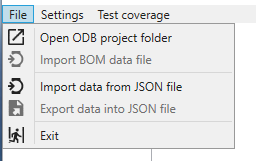
\includegraphics[width=0.4\textwidth]{images/file}
	\end{center}
	\caption{The file children menu items}
	\label{fig:02}
\end{figure}
Within the file menu item you will find the following items in order from top to bottom
\begin{itemize}
	\item Open ODB project folder - By pressing this item a new folder selection dialog will appear to make the user select any folder containing valid ODB project files
	\item Import BOM data file - This item will only be available after you have loaded a valid project into the tool and provides the possibiliy of reading out any BOM related files in order to add values to specific components
	\item Import data from JSON file - If you have exported before some valid project data into a JSON file you can import it back by using this menu item. The big advantage of using this feature is the fact that the GRPC server API for the PCB investigator doesn't need to be connected
	\item Export data into JSON file - By acting this item a new file selection dialog appears to give you the possibility of choosing a target destination for exporting all loaded data into one JSON file
	\item Exit - Close the application (But just the graphical tool, the GRPC server itself will be still running in background as it is a separate tool)
\end{itemize}

\subsection{Settings}
\begin{figure}[H]
	\begin{center}
	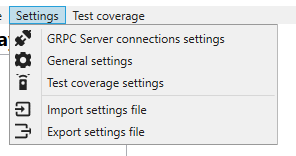
\includegraphics[width=0.4\textwidth]{images/settings}
	\end{center}
	\caption{The settings children menu items}
	\label{fig:03}
\end{figure}
Within the settings menu item you will find the follwing children items:
\begin{itemize}
	\item GRPC Server connection settings - Within this settings page you are able to define the IP address of the GRPC server API for the PCB investigator to connect to and test the connection
	\item General settings - Within this settings page you are able to define the general identifier and colors of all general components from the ODB++ project
	\item Test coverage settings - Within this page you can define all test related identifier
	\item Import settings file - The possibility of importing a previously exported settings file of this application
	\item Export settings file - The opportunity of exporting all settings into a local file for later usage
\end{itemize}

\subsection{Test coverage}
\begin{figure}[H]
	\begin{center}
	
\includegraphics[width=0.5\textwidth]{images/testCoverage}
	\end{center}
	\caption{The test coverage children menu items}
	\label{fig:04}
\end{figure}
Within this menu item you actually will just find the \textbf{Boundary scan test} menu item where you can see the following children items:
\begin{itemize}
	\item Determine all boundary scan objects - Determines in dependency on the settings from the page \textbf{Test coverage settings} all boundary scan related objects. This needs to be performed before all other operations are available
	\item Determine test coverage for JTAGs - This determines the test coverage for all interconnections directly between JTAG devices
	\item Determine test coverage for all PullUps - This determines the test coverage for all interconnections between JTAG devices and all pull up resistors
	\item Determine test coverage for all PullDonws - This determines the test coverage for all interconnections between JTAG devices and all pull down resistors
	\item Determine test coverage for all PullUps and PullDonws - This determines the test coverage for all interconnections between JTAG devices, all pull up resistors and all pull down resistors
	\item Determine test coverage for all other components - This determines the test coverage between all JTAG devices and all other components which are neither pull up nor pull down resistors
	\item Determine complete test coverage of boundary scan - This determines all previously explained tests in sum (JTAG, pull ups, pull downs and others)
\end{itemize}

\section{Working with the application}
Now a complete sequence of working with the application will be explained
\subsection{Setting up the GRPC server connection}
First of all you should either manually start the GRPC server for API with the PCB investigator or at least know its IP address of the computer where its running at. After wards you open the \textbf{Settings -> GRPC Server connections settings}
\begin{figure}[H]
	\begin{center}
	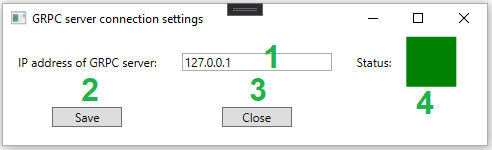
\includegraphics[width=0.5\textwidth]{images/grpcServerConnectionsSettings}
	\end{center}
	\caption{The GRPC server connections settings}
	\label{fig:05}
\end{figure}

Within this setting page you have the following possibilities:
\begin{enumerate}
	\item IP address of GRPC server - Here you should type in the IP address of the computer where the server is running at
	\item Save - By pressing this button the IP address will be saved and a connection try is being performed. If connection was successful then the painting area \textbf{3} will be painted in green otherwise in red
	\item Close - Close this settings window without saving the changes made
	\item Status - The connection status to the server (Green if successful otherwise red)
\end{enumerate}

\subsection{Setting up the general settings}
\begin{figure}[H]
	\begin{center}
	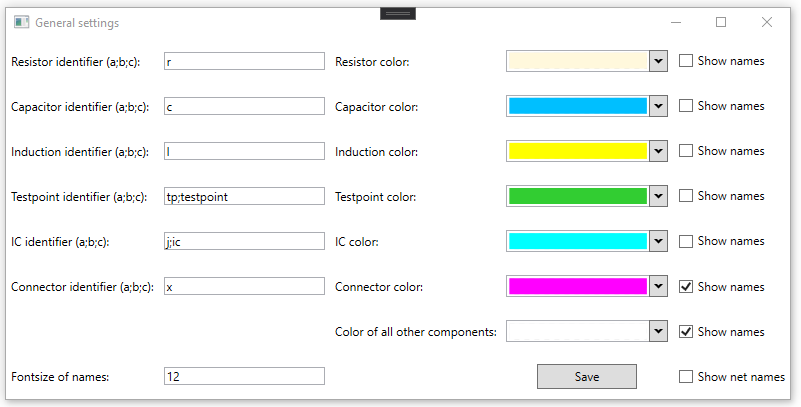
\includegraphics[width=0.7\textwidth]{images/generalSettings}
	\end{center}
	\caption{The general settings}
	\label{fig:05}
\end{figure}
By opening next the \textbf{Settings -> General settings} you will have the possibility of defining the following values:
\begin{itemize}
	\item Resistor identifier (a;b;c) - The semicolon separated identifier for detecting resistors by its name
	\item Resistor color - The color to be used for painting resistors
	\item Capacitor identifier (a;b;c) - The semicolon separated identifier for detecting capacitors by its name
	\item Capacitor color - The color to be used for painting capacitors
	\item Induction identifier (a;b;c) - The semicolon separated identifier for detecting inductions by its name
	\item Induction color - The color to be used for painting inductions
	\item Testpoint identifier (a;b;c) - The semicolon separated identifier for detecting testpoints by its name
	\item Testpoint color - The color to be used for painting testpoints
	\item IC identifier (a;b;c) - The semicolon separated identifier for detecting ICs by its name
	\item IC color - The color to be used for painting ICs
	\item Connector identifier (a;b;c) - The semicolon separated identifier for detecting connectors by its name
	\item Connector color - The color to be used for painting connectors
	\item Color of all other components - The color to be used for all other unidentified components
	\item Fontsize of names - The font size to be used for displaying the names of components
	\item Show all net names - If enabled then all net names will be displayed between active connections of components
	\item Save - Save all changes and close the window
\end{itemize}

\subsection{Opening a ODB++ project}
By clicking on \textbf{File -> Open ODB project folder} a new folder selection dialog will appear where you have the possibility of choosing any valid ODB++ project. After you selected one and confirmed the selection the following loading animation will be displayed for the time all data is being transferred by the GRPC server and parsed into that application:
\begin{figure}[H]
	\begin{center}
	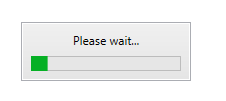
\includegraphics[width=0.5\textwidth]{images/loadingAnimation}
	\end{center}
	\caption{The loading animation}
	\label{fig:06}
\end{figure}

\subsection{Import BOM data file}
\begin{figure}[H]
	\begin{center}
	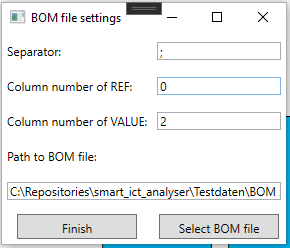
\includegraphics[width=0.5\textwidth]{images/bomFile}
	\end{center}
	\caption{Import BOM data file}
	\label{fig:06a}
\end{figure}
By clicking on the menu item \textbf{File -> Import BOM data file} a new window appears and allows you to define the following values:
\begin{itemize}
	\item Separator - As the BOM files are typically CSV files you have to define the separator here is being used within that file
	\item Column number of REF - The column number (beginning with 0) where the REF, the component name is specified
	\item Column number of VALUE - The column number (beginning with 0) where the according value to a components name is specified
	\item Path to BOM file - The actual selected filepath to the file to be imported as BOM file
	\item Select BOM file - By clicking on this button a new file open dialog will appear to give you the possibility of choosing any file which its location then will be displayed in the field above
	\item Finish - Trigger the importing process of BOM data
\end{itemize}

\begin{figure}[H]
	\begin{center}
	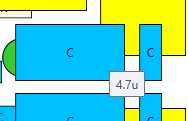
\includegraphics[width=0.5\textwidth]{images/values}
	\end{center}
	\caption{Values of components by hovering over them with mouse}
	\label{fig:06a}
\end{figure}

After successfully importing of a BOM file you should now be able to hover with the mouse over any component to see its value which was imported before. All components which does not have any values specified within the BOM file will be bordered in red color:

\begin{figure}[H]
	\begin{center}
	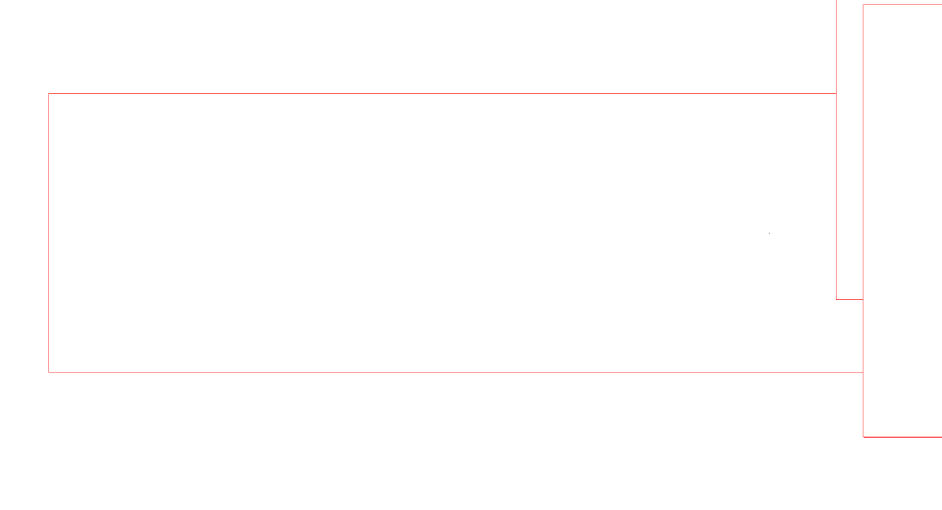
\includegraphics[width=0.5\textwidth]{images/redBordered}
	\end{center}
	\caption{Red bordered components without any values from BOM file}
	\label{fig:06a}
\end{figure}

\subsection{Selection of layers for representation}
After a project was loaded successfully you should then see at least one entry within the layers section of the application. By selecting one or more layers the respective objects of these selected layers will be painted into the painting area:
\begin{figure}[H]
	\begin{center}
	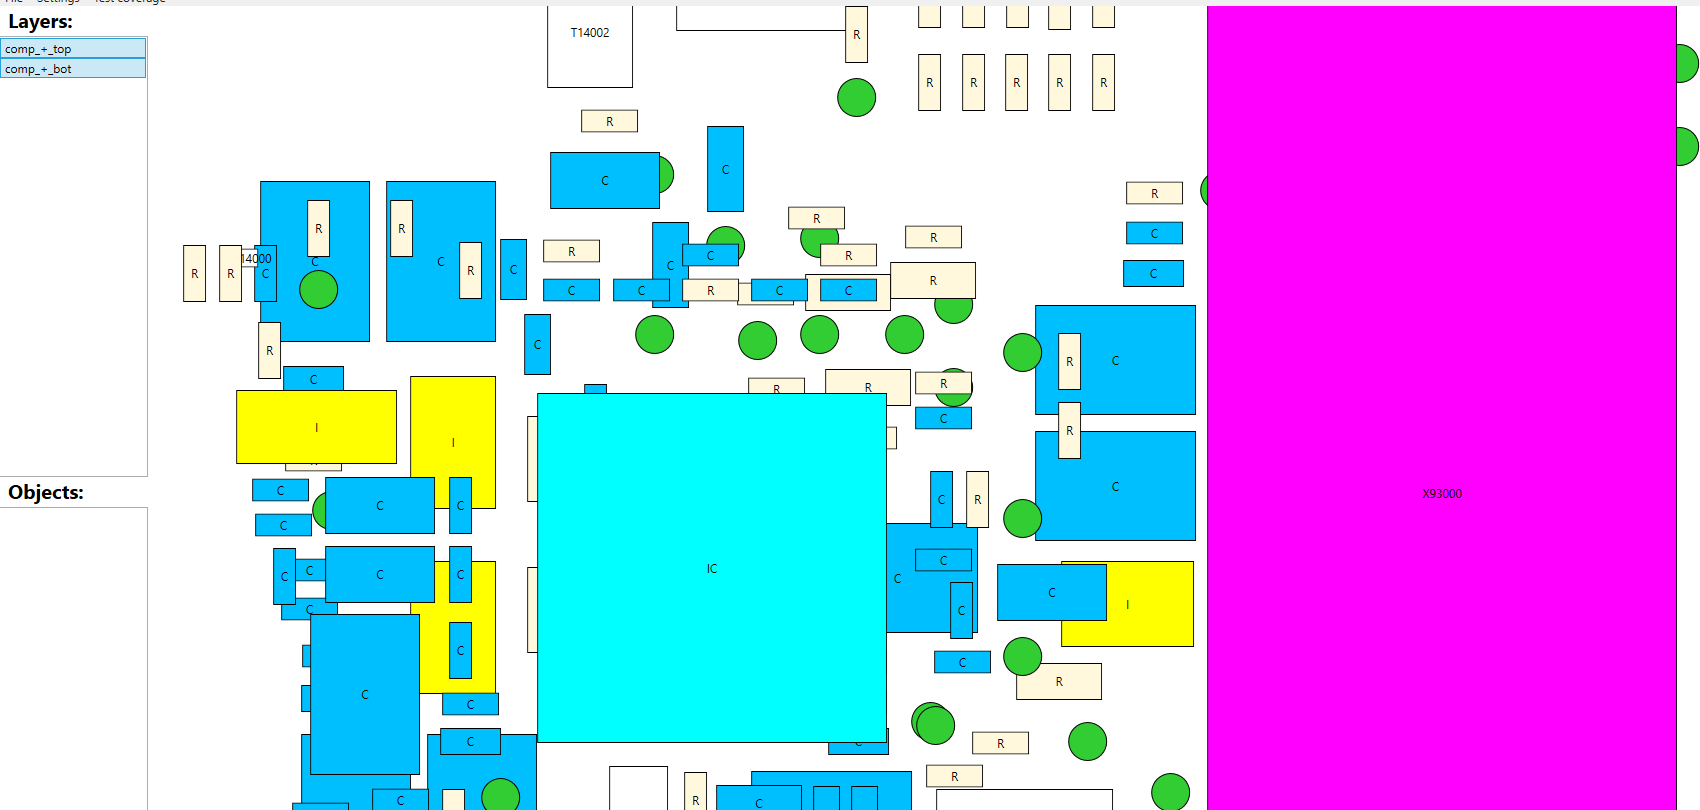
\includegraphics[width=0.5\textwidth]{images/paintedArea}
	\end{center}
	\caption{The area filled with selected layer objects}
	\label{fig:06}
\end{figure}

Within this painting area you have now these possibilites of actions:
\begin{itemize}
	\item Mouse scrolling - By scrolling up the mouse wheel the zoom will be increased and by scrolling down the mouse wheel the zoom will be decreased
	\item Right click on any object of representation
	\begin{itemize}
		\item Toggle visibility - Shows any object in transparent or not transparent way
		\item Toggle visibility of all objects with the same type - Shows all objects of the same type as selected in transparent way or not
		\item Toggle display of connections - Shows all connections to other objects as lines or not
	\end{itemize}
\end{itemize}

\subsubsection{Toggle visibility}
\begin{figure}[H]
	\begin{center}
	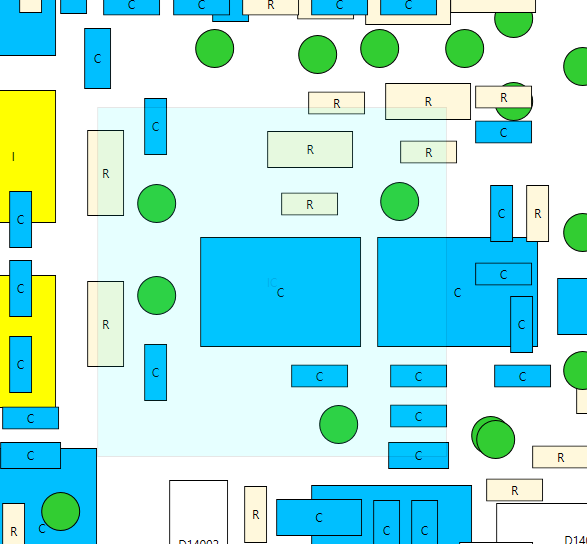
\includegraphics[width=0.5\textwidth]{images/toggleVisibility}
	\end{center}
	\caption{Toggle visibility of one object}
	\label{fig:07}
\end{figure}

As shown only the selected object will be painted in transparent way if \textbf{Toggle visibility} was performed. In that way you are able to see all objects which were covered by that specific object before

\subsubsection{Toggle visibility of all objects with the same type}
\begin{figure}[H]
	\begin{center}
	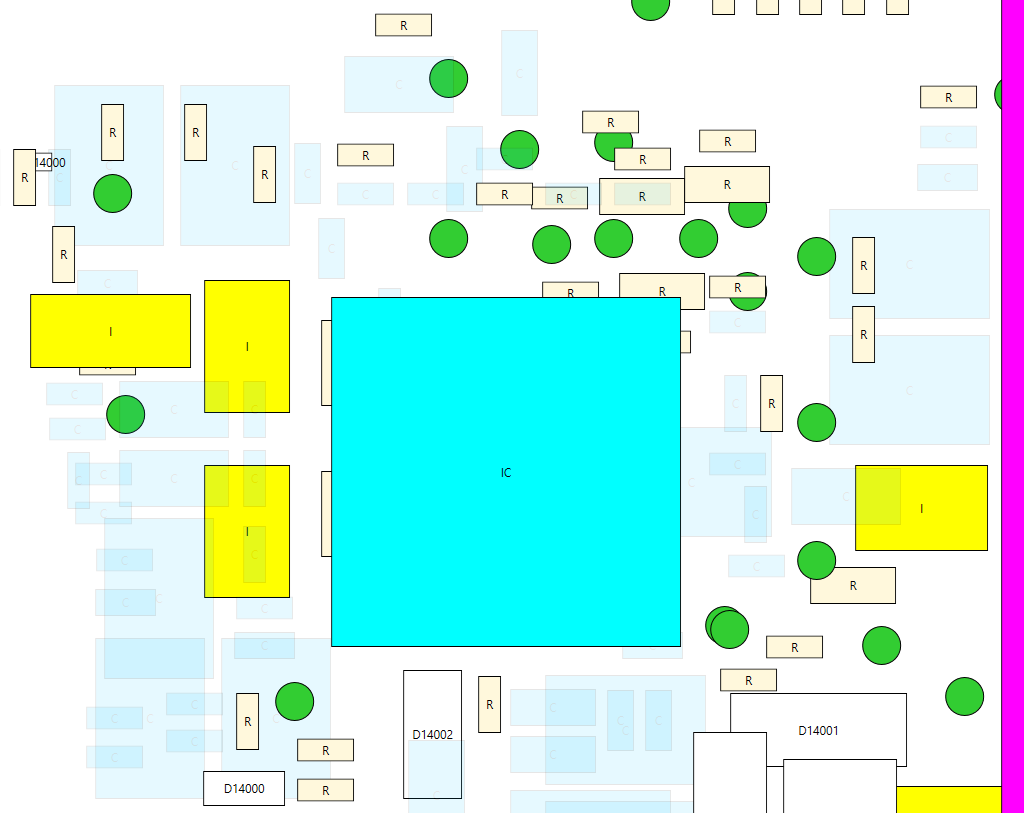
\includegraphics[width=0.5\textwidth]{images/toggleVisibilityAll}
	\end{center}
	\caption{Toggle visibility of all objects with the same type}
	\label{fig:08}
\end{figure}

The same result as by performing the action \textbf{Toggle visibility} but just for every object of the same type

\subsubsection{Toggle display of connections}
\begin{figure}[H]
	\begin{center}
	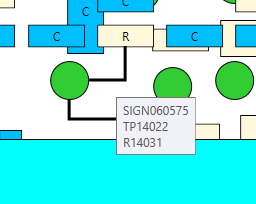
\includegraphics[width=0.5\textwidth]{images/connections}
	\end{center}
	\caption{Toggle display of connections}
	\label{fig:09}
\end{figure}

By performing \textbf{Toggle display of connections} all availabe connections of that selected object will be displayed as lines. Furthermore you have the possibility of hovering over any line to get these information:
\begin{itemize}
	\item The netname of interconnections
	\item The name of the first object (The selected one)
	\item The name of the second object
\end{itemize}

\subsubsection{Show net names}
\begin{figure}[H]
	\begin{center}
	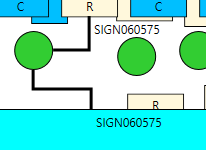
\includegraphics[width=0.5\textwidth]{images/netnames}
	\end{center}
	\caption{Show net names}
	\label{fig:10}
\end{figure}
If the option \textbf{Show net names} will be enabled then after toggling the visible connections furthermore all net names will be displayed

\subsection{Determine all boundary scan objects}
\begin{figure}[H]
	\begin{center}
	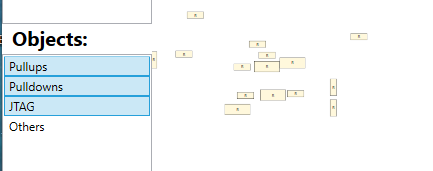
\includegraphics[width=0.5\textwidth]{images/determinigTestCoverageObjects}
	\end{center}
	\caption{Object types for boundary scan test}
	\label{fig:11}
\end{figure}
After you performed the \textbf{Test coverage -> Boundary scan test -> Determine all boundary scan objects} action the following types will be selectable for being displayed within the painting area:
\begin{itemize}
	\item Pullups - All pull up resistors of the project
	\item Pulldowns - All pull down resistors of the project
	\item JTAG - All JTAG related devices of the project
	\item Others - All other objects which are connected to the JTAG devices
\end{itemize}

\subsubsection{Perform any test for determining the test coverage}
\begin{figure}[H]
	\begin{center}
	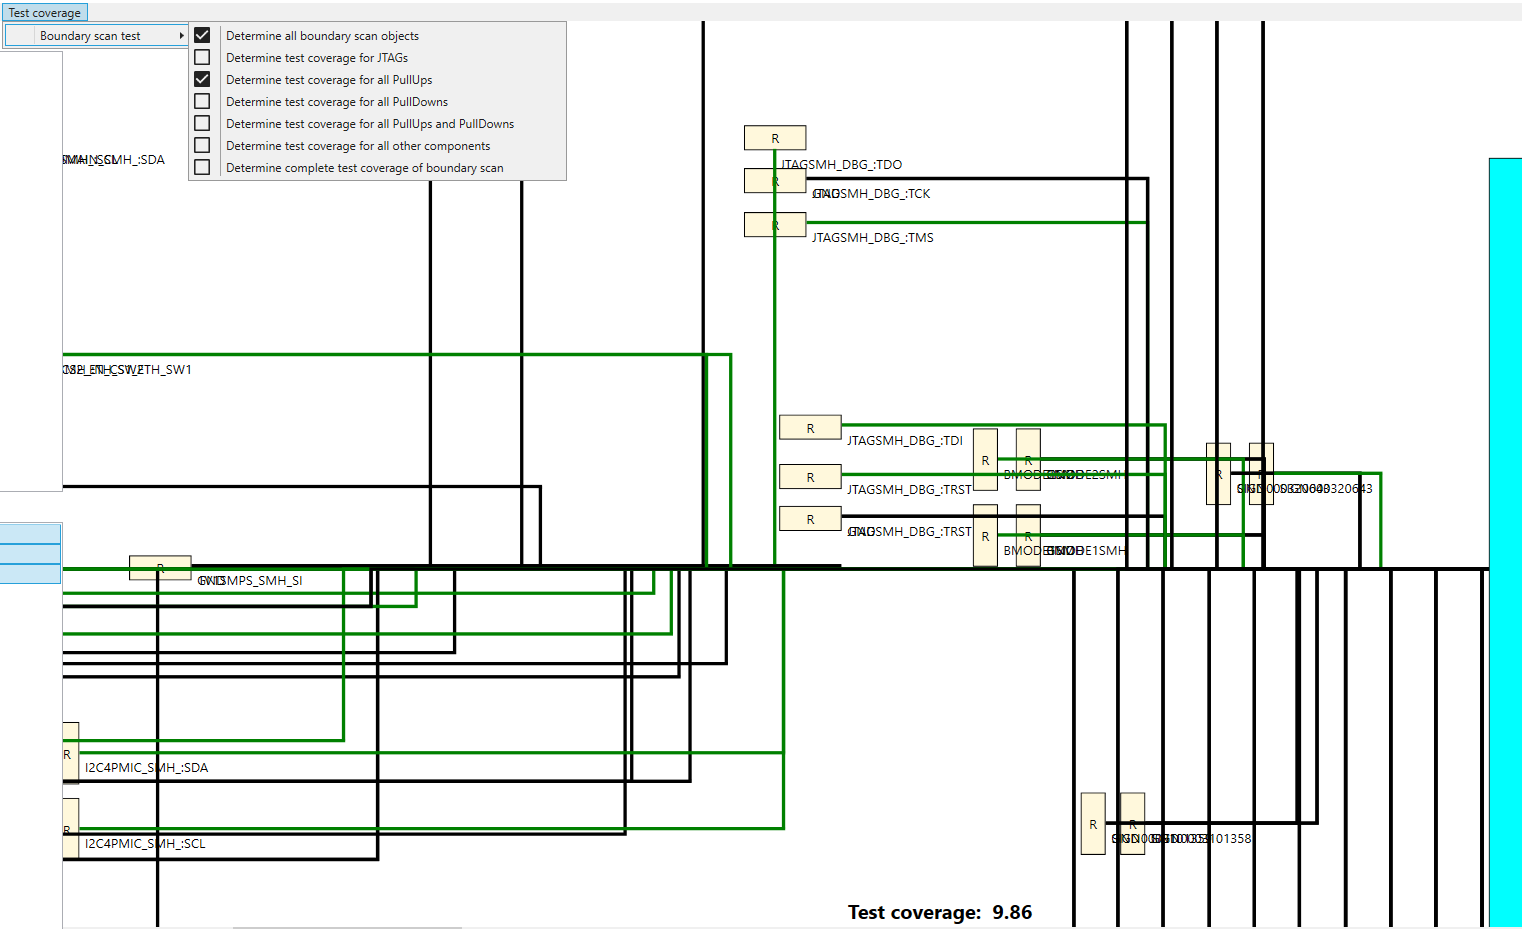
\includegraphics[width=0.5\textwidth]{images/testCoverageOfAllPullUps}
	\end{center}
	\caption{Test coverage of all pull ups}
	\label{fig:10}
\end{figure}
After you performed any test (in this example it was the test coverage for all pull ups) then the according check box to the menu item will be checked. That means if it was before unchecked then it will be checked and the other way around. Now for all components which check boxes are checked all connections of the JTAG devices will be painted in green. And finally a textual representation of the test coverage result is being displayed in the bottom area.

\subsection{Export data into JSON file}
After or during work with the project you shouldn't forget to export all data into a JSON file to have the possibility of loading it much faster and without the dependency on setting up the GRPC server connection.

\newpage
\section{Acroyms}
PullUps - Pull up resistors which are directly connected to a power supply
PullDowns - Pull down resistors which are directly connected to ground connection
JTAG - Joint Test Action Group (A connection device with the possibility of advanced electrical testing mechanisms)
IC - Integrated circuit (A complex component consisting of many connections and other internal components)

\newpage

% RevisionHisory
\begin{versionhistory}
\vhEntry{1.0.0}{10.02.2021}{RAM}{Initial version of documentation}
\vhEntry{1.0.1}{14.04.2021}{RAM}{Overworked complete content by using new style of tool}
\end{versionhistory}
\end{document}

% End Document